\section{Final Assignment}

For the final assignment, I am managing a database using SQL and the ESP32.
I chose for this assignment because of the likelihood that the ESP32 has to interact with a database for the final product.
The goal of this assignment is to make the ESP32 able to log certain events, which will be stored into a database.
The event that will be logged is the pressing down of a push button.
The ESP32 will not communicate directly with the database; instead, it communicates with the database via a web server.
This is removes the need for the ESP32 to run a heavy SQL client and instead a much simpler HTTP client can be used.

\subsection{Demonstration Setup}

\begin{figure}[htbp]
    \centering
    \begin{circuitikz}
        \ctikzset{multipoles/dipchip/pin spacing=0.2}
        \ctikzset{resistor=european}
        \draw (0,0) node[dipchip,
            num pins=30,
            hide numbers,
            external pins width=0.1,
            external pad fraction=3](C){ESP32};

            \draw (C.pin 15) -- ++(-0.5,0) -- ++(0,-0.5) -- ++(3,0) -- ++(0,5) -- ++(-3,0) coordinate (P1);
            \draw (C.pin 14) -- ++(-0.5,0) to[R] ++(-2.0,0) -- ++(0,1.5) to[push button] ++(0,1) coordinate (P2) -- (P2|-P1) -- (P1);
            \draw (C.pin 11) -- ++(-2.5,0);

            \node [right,font=\tiny]
            at (C.bpin 11) {GPIO27};

            \node [right,font=\tiny]
            at (C.bpin 14) {GND};

            \node [right, font=\tiny]
            at (C.bpin 15) {5V};
    \end{circuitikz}
    \caption{Electric Circuit}
\end{figure}

\noindent
I used the circuit above to connect the push button to the ESP32.
The locations of the pins may differ depending on which version of the ESP32 is being used.
As for setting up the software, the client is flashed onto the ESP32 and the web server and the database are hosted a Raspberry Pi.
I configured port forwarding on my home network (where the Raspberry Pi is connected to) so that the ESP32 also can communicate with the web server from other networks.

\subsection{Development Environment and Tooling}

For programming the ESP32, I decided on using the ESP-IDF.
I have used the \code{idf.py} command-line tool for building and flashing the project.
For configuring the web server and database I used OpenSSH, to establish a SSH connection.
I wrote the code using the Vim text editor and used Git for version control.

\subsection{Used Software Libraries}

\subsubsection{Client}

For the client, I have used libraries that come with ESP-IDF.
These libraries allowed me among other things to establish a \gls{wifi} connection and perform \gls{http} requests.
No third-party libraries were used.

\subsubsection{Server}

For the server, I have used Go's standard library packages for working with \gls{http} and SQL.
However, Go's standard library package \href{https://pkg.go.dev/database/sql}{database/sql} does not work with MySQL out of the box.
I had to use a third-party package that contains a MySQL driver that implements the \href{https://pkg.go.dev/database/sql/driver}{database/sql/driver} interface \cite{go-mysql-driver}.
%I had to use another package that enables MySQL support for Go's \href{https://pkg.go.dev/database/sql}{database/sql} standard library package.
%This package contains a Go driver for MySQL and can be found at: \url{https://github.com/go-sql-driver/mysql}.

\subsection{Software Architecture}

\subsubsection{Basic Architecture}

The software consists of three major components: a \gls{http} client, a \gls{http} server, and a relational database.
The ESP32 is communicating with the web server and the web server communicates with the database.
The client makes \gls{http} requests to the server, after which the server will query the database based on the request being made.
The source code can be found on \href{https://github.com/jochemarends/project-integration/tree/main/final-assignment}{GitHub} \cite{github-final-assignment}.
%There are two types of request that can be made: one for creating new users and another one for logging events.

\begin{figure}[H]
    \begin{center}
    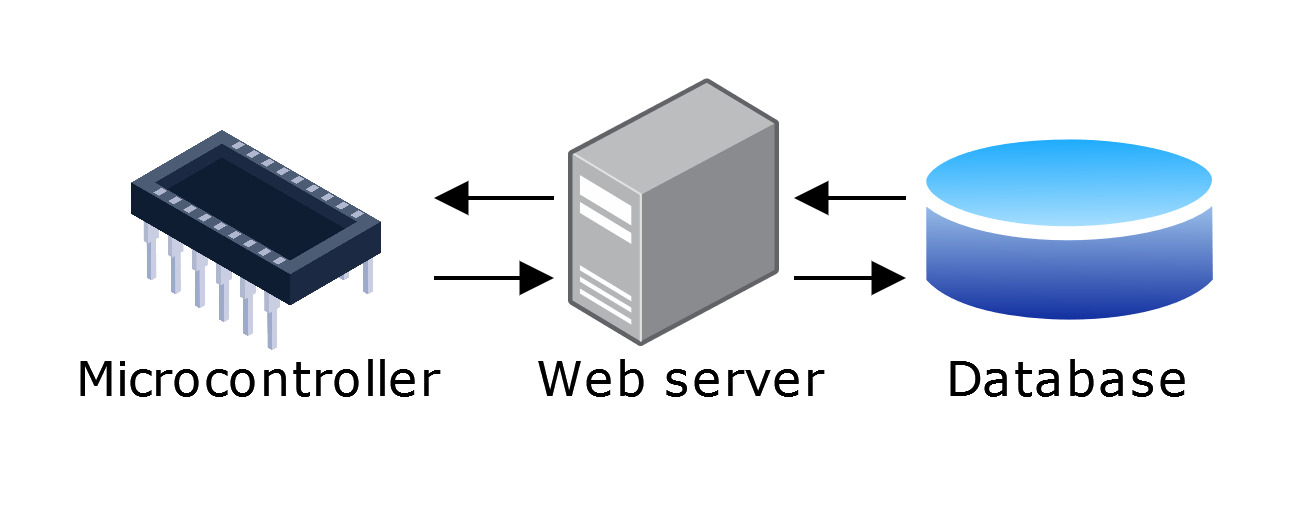
\includegraphics[width=\textwidth]{images/architecture-diagram}
    \end{center}
    \caption{Basic Architecture Diagram}
\end{figure}

\subsubsection{Database}

The database is managed using MySQL, I have put the \gls{erd} of the database below.
A patient has a unique ID and a name, however, some additional information may be stored along this.
Logs can be created that belong to a specific patient.
The "Log" table contains a "kind" field, to account for the possibility of other events being added in the future.

\begin{figure}[H]
    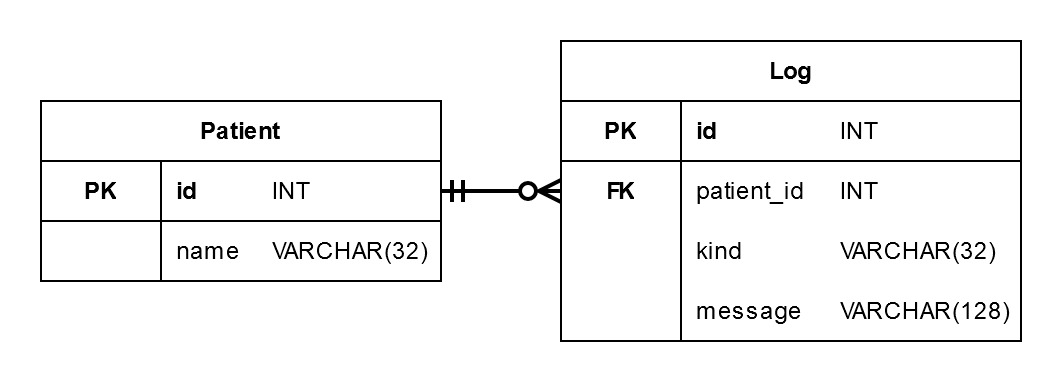
\includegraphics[width=\linewidth]{images/erd}
    \caption{Entity Relationship Diagram}
\end{figure}

%\noindent
%\begin{minipage}{0.45\textwidth}
%    The database is managed using MySQL, I have put the \gls{erd} of the database below.
%    A patient has a unique ID and a name, however, some additional information may be stored along this.
%    Logs can be created that belong to a specific patient.
%    The "Log" table contains a "kind" field, to account for the possibility of other events being added in the future.
%\end{minipage}
%\hfill
%\begin{minipage}{0.55\textwidth}
%    \begin{figure}[H]
%        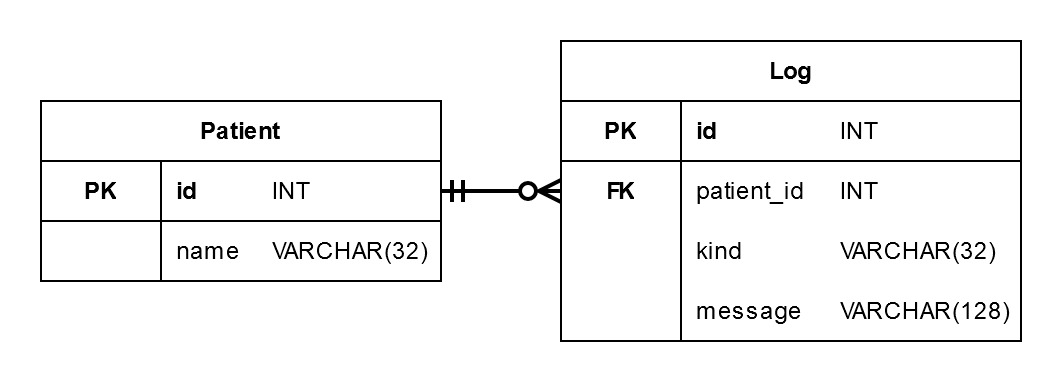
\includegraphics[width=\linewidth]{images/erd}
%        \caption{Entity Relationship Diagram}
%    \end{figure}
%\end{minipage}

\subsubsection{Web Server}

The \gls{http} server provides two services: registering new patients and the logging events.
Arguments are passed using form field. In the table below, the services are briefly documented.

\begin{center}
    \begin{tabular}{l|l|l|l}
        Service & Path & Form Field(s) & Returns \\
        \hline
        Register Patient & \texttt{/add-patient} & \texttt{name=\textit{name}} & An ID unique to the patient. \\
        \hline
        Log Event & \texttt{/log-event} & \texttt{id=\textit{id}\&msg=\textit{msg}} & - \\
    \end{tabular}
    \captionof{table}{Brief Description of Services}
\end{center}

\noindent
Below two flowchart can be seen, one for each service.
The two are almost identical to each other, but the queries they perform are different.
Also, the flowchart on the right side does not explicitly return data. 
Both flowcharts are used as submodule in the client's flowchart.

\begin{figure}[H]
    \begin{center}
    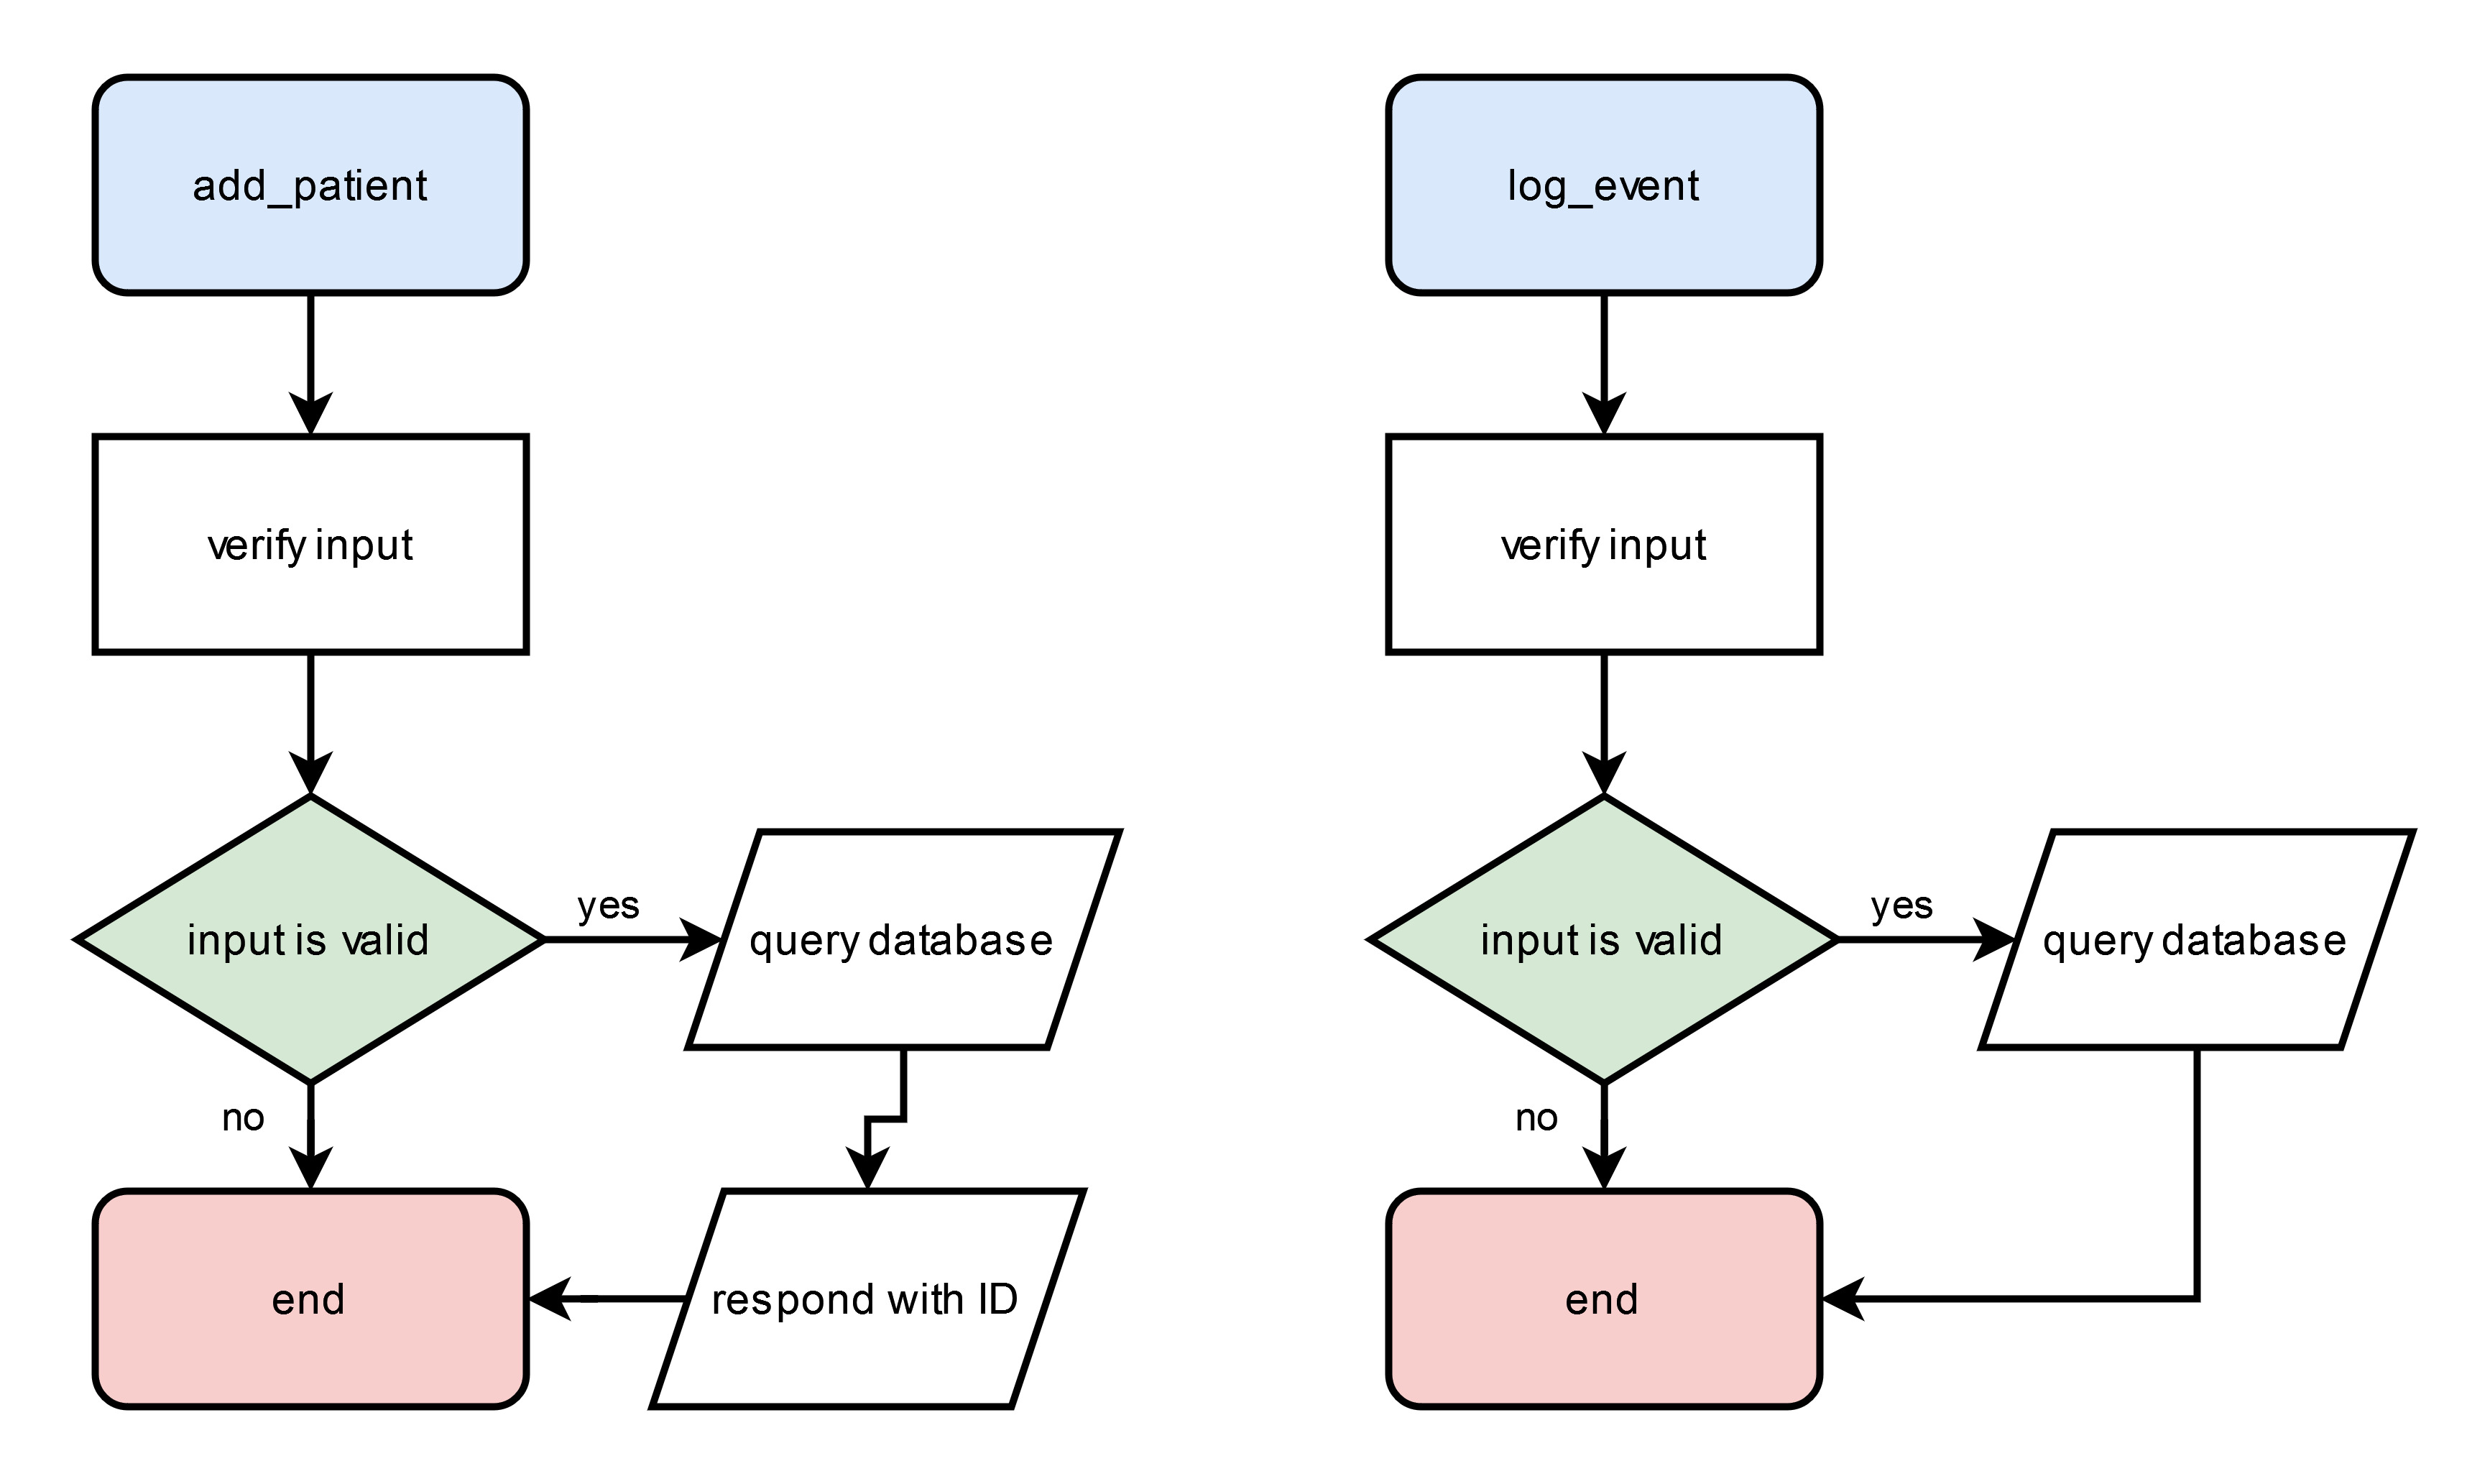
\includegraphics[width=\textwidth]{images/flowchart-server}
    \end{center}
    \caption{Flowchart of Server}
\end{figure}

\subsubsection{Client}

Upon booting, the client registers a new a patient by making a \gls{http} request to the web server.
After this, the client will check for a button press, if one occurred, a new \gls{http} request will be made for logging the event.
A flowchart for the client can be seen below.

\begin{figure}[H]
    \begin{center}
    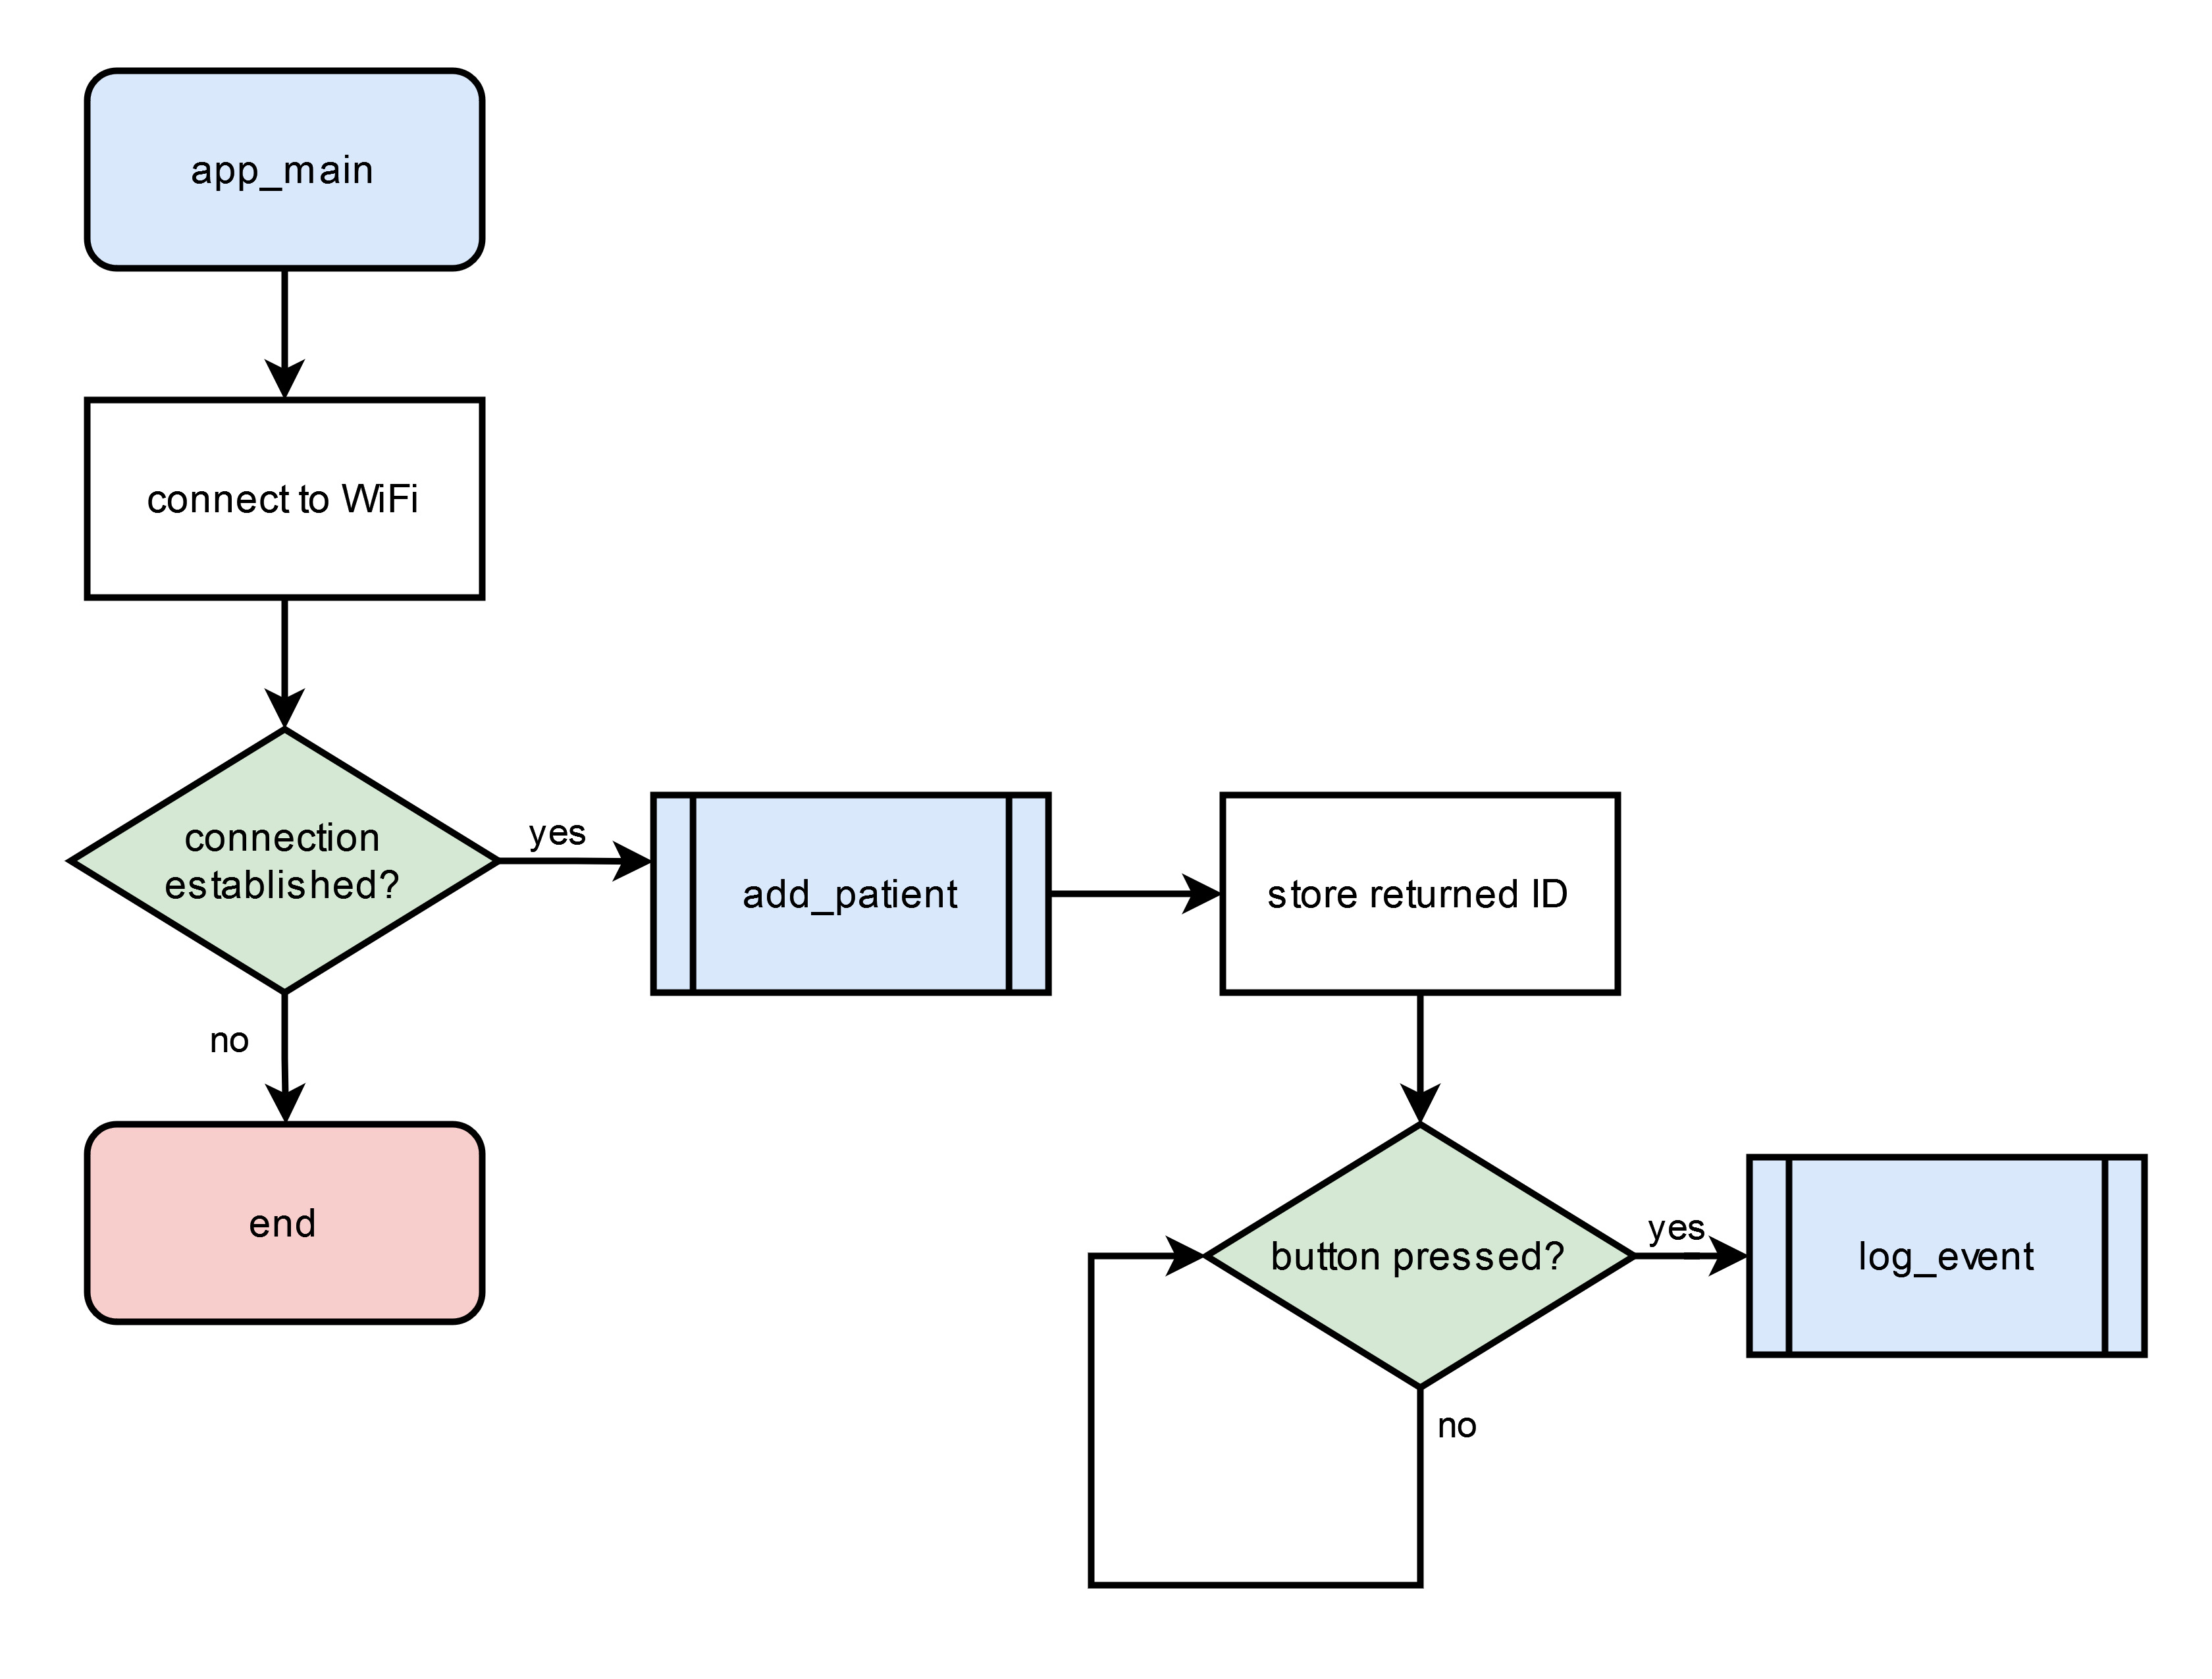
\includegraphics[width=\textwidth]{images/flowchart-client}
    \end{center}
    \caption{Flowchart of Client}
\end{figure}

%Of these components, the  server and the database are hosted a Raspberry Pi, while the  client runs on an ESP32.
%The \gls{http} client communicates with the \gls{http} server, which in turn communicates with the database.
%The ESP32 is interacting with the database via a web server as hosting a SQL client would be a very intensive task for a microcontroller.

\subsection{Results}

At first instance, I wanted to query the database directly from the ESP32.
However, soon found out that this was not a trivial task as it would require the ESP32 to run a SQL client.
I decided on using a web server, which I think is a better solution since it encapsulates access to the database and prevents one from performing malicious queries.
This was the only challenge I have encountered.

\subsection{Reccomendations}

If I were to continue working on this small project, I would change several things. 
I would add some sort of authentication to prevent anyone from inserting data for arbitrary patients.
Additionaly, I would change the client, so it would refrain from registrating a new user every time it boots.
Lastly, I would add timestamps to the logs.

\subsection{Accountability}

I have done this assignment by myself.

\clearpage

